\documentclass[10pt,twocolumn,letterpaper]{article}
%% Welcome to Overleaf!
%% If this is your first time using LaTeX, it might be worth going through this brief presentation:
%% https://www.overleaf.com/latex/learn/free-online-introduction-to-latex-part-1

%% Researchers have been using LaTeX for decades to typeset their papers, producing beautiful, crisp documents in the process. By learning LaTeX, you are effectively following in their footsteps, and learning a highly valuable skill!

%% The \usepackage commands below can be thought of as analogous to importing libraries into Python, for instance. We've pre-formatted this for you, so you can skip right ahead to the title below.

%% Language and font encodings
\usepackage[english]{babel}
\usepackage[utf8x]{inputenc}
\usepackage[T1]{fontenc}
\usepackage{graphicx}
\usepackage{subfigure}
\usepackage{natbib}
\usepackage{listings}
\usepackage{booktabs}
\usepackage{algorithm}
\usepackage{algorithmic}
\usepackage{amsfonts}
\usepackage{cuted}


%% Sets page size and margins
\usepackage[a4paper,top=3cm,bottom=2cm,left=3cm,right=3cm,marginparwidth=1.75cm]{geometry}

%% Useful packages
\usepackage{amsmath}
\usepackage[colorinlistoftodos]{todonotes}
\usepackage[colorlinks=true, allcolors=blue]{hyperref}
\usepackage{natbib}
\bibliographystyle{unsrt}

\definecolor{blve}{rgb}{0.3372549 , 0.61176471, 0.83921569}
\definecolor{gr33n}{rgb}{0.29019608, 0.7372549, 0.64705882}
\makeatletter
\lst@InstallKeywords k{class}{classstyle}\slshape{classstyle}{}ld
\makeatother
\lstset{language=C++,
	basicstyle=\ttfamily,
	keywordstyle=\color{blve}\ttfamily,
	stringstyle=\color{red}\ttfamily,
	commentstyle=\color{magenta}\ttfamily,
	morecomment=[l][\color{magenta}]{\#},
	classstyle = \bfseries\color{gr33n}, 
	tabsize=2
}
\lstset{basicstyle=\ttfamily}


%% Title
\title{
		\usefont{OT1}{bch}{b}{n}
		\normalfont \normalsize \textsc{CS121 Parallel Computing Lab 2} \\ [10pt]
		\huge Cuckoo Hashing using CUDA \\
}
\selectlanguage{english}
\usepackage{authblk}
\author[]{Hongtu Xu, 2019533229}
\affil[]{xuht1@shanghaitech.edu.cn}


\begin{document}
\maketitle

\begin{abstract}

In computing, a hash table is a widely used data structure that implements an associative array abstract structure, a structure that maps keys to values. Cuckoo Hashing is one among the hashing techniques which provides high memory usage with constant time access \cite{Chadalavada2017ImprovingCH}. At the same time, GPU makes high throughput hash table possible. In this lab, I implement Cuckoo Hashing use CUDA as well as testing correctness and doing experiments to analyze performance.

\end{abstract} 

\section{Introduction}
\subsection{Compile \& Build}

You need a C++ compiler which supports at least C++ 17 standard and nvcc which supports at least C++ 17 standard for CUDA C++.\\
I use CMake to build the project, so you also need to have CMake with version at least 3.21 to compile our codes.\\
Compile by:
\begin{lstlisting}[language=bash]
mkdir build
cd .\build
cmake ..
cmake --build . --config Release
\end{lstlisting}
Run the benchmark by main target under tests:
\begin{lstlisting}[language=bash]
cd .\build\tests
.\main.exe
\end{lstlisting}
It will automatically run the four experiments with an additional correctness test.

\subsection{Interface}

We provide a function insert\_and\_lookup to use our hash table. \\
It will first insert the given keys into the hash table and then do the lookup and store the result according to the given lookup key sequence.

\subsection{Benchmark Configures}

I run my code on my own computer. The detailed information are:

\begin{table}[h]
\begin{tabular}{@{}c|c@{}}
\toprule
Config   & Value                                             \\ \midrule
CPU      & AMD Ryzen 7 3700X \\
GPU     &  NVIDIA GeForce RTX 2060 SUPER \\ 
Memory   & 32 GB DDR4 3000 MHz 2 of 4 slots                                            \\
GPU Memory & 8 GB GDDR6  \\
OS       & Windows 11 Pro 22000.37                                  \\
Compiler &  MSVC 19.30.30706, nvcc V11.5.119                                  \\
Optimize & MSVC: /O2, nvcc: -O3                                              \\ 
CUDA Cores   & 2176 \\
CUDA Version & 11.5 \\
Driver Version & GeForce Game Ready Driver 497.29 \\
\bottomrule
\end{tabular}
\end{table}

To test scalability, I also run my code on a cloud virtual machine provided by tencent cloud. The detailed information are:

\begin{table}[h]
\begin{tabular}{@{}c|c@{}}
\toprule
Config   & Value                                             \\ \midrule
CPU      &  AMD EPYC $\text{ROME}^{\text{TM}}$ 7k62 (16 vCPU) \\
GPU     &  NVIDIA TESLA A100 40GB PCIe \\ 
Memory   & 96 GB                                             \\
GPU Memory & 40 GB HBM2e  \\
OS       & Ubuntu 20.04 LTS                                  \\
Compiler &  gcc 11.1.0, nvcc V11.1.105                                  \\
Optimize & gcc: -O2, nvcc: -O3                                              \\ 
CUDA Cores   & 6912 \\
CUDA Version & 11.1 \\
Driver Version & 450.102.04 \\
\bottomrule
\end{tabular}
\end{table}

\section{Implement Details}

\subsection{Cuckoo Hashing Algorithm}

Cuckoo Hashing is one of the hash table schemas which provides high memory utilization and constant access time \cite{Chadalavada2017ImprovingCH}. It is named after a type of bird who lays its eggs in other birds' nests, and whose chicks push out the other eggs from the nest after they hatch. \\
Unlike many other hash tables, Cuckoo Hashing uses $t$ hash functions where $t > 1$. Cuckoo hashing maintains $t$ tables, each key $k$ can be stored into $t$ locations corresponds to the location that uses hash function $h_i$.
In the insertion process, suppose we want to insert a key $k$ into the hash table and we have $t$ hash functions $h_0, h_1, \cdots, h_{t - 1}$ while the tables are $T_0, T_1, \cdots, T_{t - 1}$. We will first use hash function $h_1$ to try to insert $k$ into $T_1[h_1(k)]$. If the cell is already occupied, then we will evict the key in that slot $k'$, put the $k$ into that cell and try to insert $k'$ into tables after circularly. If we still need to evict key after a bound times, then we need to choose some other functions and rehash.\\
\begin{algorithm} 
	\caption{Cuckoo Hashing Insert} 
	\label{basic_insert} 
	\begin{algorithmic}
	    \STATE $h_1, h_2, \cdots, h_t$ are $t$ hash functions
	    \STATE $T_1, T_2, \cdots, T_t$ are corresponding tables
	    \STATE $C$ is the size of the table (capacity)
	    \STATE \textbf{input:} a key $k$
	    \FOR{$i = 0 \to \text{iter-bound}$}
	        \STATE $\text{loc} \gets h_{i \bmod t}(k) \bmod C$
	        \IF{$T_{i \bmod t}[\text{loc}] = \text{empty}$}
	            \STATE $T_{i \bmod t}[\text{loc}] \gets k$
	            \RETURN
	        \ELSE
	            \STATE $\text{swap}(k, T_{i \bmod t}[\text{loc}])$
	        \ENDIF
	    \ENDFOR
	    \STATE rehash()
	    \STATE insert($k$)
	\end{algorithmic} 
\end{algorithm}\\
The lookup process is much simpler, we just need to loop through all $t$ possible locations and compare the key with the stored key in the table whether they are equal. Obviously, this process is done in $O(t)$ and since $t$ is a constant, then Cuckoo Hashing provides constant time access.

\begin{algorithm}
    \caption{Cuckoo Hashing Lookup}
    \label{basic_lookup}
    \begin{algorithmic}
        \STATE $h_1, h_2, \cdots, h_t$ are $t$ hash functions
	    \STATE $T_1, T_2, \cdots, T_t$ are corresponding tables
	    \STATE $C$ is the size of the table (capacity)
	    \STATE \textbf{input:} a key $k$
	    \FOR{$i = 0 \to t - 1$}
	        \STATE $\text{loc} = h_i(k) \bmod C$
	        \IF{$T_i[\text{loc}] = k$}
	            \RETURN true
	        \ENDIF
	    \ENDFOR
	    \RETURN false
    \end{algorithmic}
\end{algorithm}

We can find that the lookup time in Cuckoo Hashing is $O(t) = O(1)$, which is very good. But the worst case exists when key is not inserted into the hash table, it will loop through all $t$ hash functions.

\subsection{Table Storage}

Since Cuckoo Hashing needs to maintain $t$ tables where $t$ is the number of hash functions. From the algorithm, it is obvious that the tables are independent to each other. So, instead of storing all the $t$ tables into a big linear array, we choose to store $t$ linear arrays, which performs better because of good pipeline and cache utilization.

\subsection{Memory Management}

For hash table, we mainly need some big linear arrays. Although unified memory can greatly decrease the difficulty for memory management between device and code. But it needs some techniques to achieve good performance and it may still perform a little bit worse than directly manage host and device memory. Therefore, I create a class to encapsulate cuda array. By overloading assignment operator, I can make copy operation between device and host simpler. Also, by encapsulation, I can allocate and free the memory by some class methods easily. 

\subsection{Random Set Generation}

We need to generate random set to test our hash table. Since it is a set which means it cannot contain the same value, then I choose to first generate a such set on CPU and then copy it to GPU. I use std::mt19937, a mersenn twister engine, as our random number engine. To make the generation faster, I create a bitset whose size is $2^{32}$, which will cost $0.5$ GB memory but provides much better performance than using a hash table to filter out duplicates. \\
For the lookup set generation, I first generate a totally different set respected to the original random set with the same size. Then, I implement a random shuffle kernel function to support shuffle operation on a device array. For the lookup set, I will first shuffle it randomly then overwrite some keys using elements from the different set according to the given percentage. This is much faster than using bitset or hash table to filter and create another set.

\subsection{Multi-level Table}

One possible method to improve the performance of our GPU hash table is to use multi-level table \cite{analysinghashtable}. The bottleneck of Cuckoo Hashing is memory access, uncoalesced global memory access will greatly influence our performance. So, we may create multi-level tables. For example, two-level Cuckoo Hashing, we first hash the elements into different buckets and then perform Cuckoo Hashing locally inside those buckets.\\
This often performs better than single-level table when needing rehashing. However, in our experiments, we do not need to rehash that much and according to the result in \cite{analysinghashtable}, the multi-level table performs even worse than single-level. Therefore, I choose to not use multi-level table and in my experiments, I compared my code with an existing multi-level cuckoo hashing code and I performs much better than him.

\subsection{Parallel d-Pipeline}

During researching, I found another way to increase the throughput, which is parallel d-pipeline \cite{7070722}. Consider the insertion process of one key $k$, it will go through tables like a pipeline:
$$\text{input} \rightarrow T_0 \rightarrow T_1 \rightarrow T_2 \rightarrow \cdots \rightarrow T_{t - 1} \rightarrow \text{rehash}$$
If success at one table in the middle, it will jump out the pipeline. Therefore, when a key failed at $T_0$ and evict one to try to insert in $T_1$, another new key can start to insert at $T_0$ without any race condition. And this forms a pipeline.\\
However, implement this directly is hard in coding. Hopefully, by taking advantage of modern compiler and C++ we can form the pipeline using template metaprogramming to expand the code and finally form a good pipeline through compiler optimization.

\subsection{Hash Function}

Since Cuckoo Hashing has a constant lookup time, then we just need to focus on insertion. A good hash function can cause less collisions and thus we can perform fewer evictions and finally gain a better performance in insertion.

\subsubsection{Universal Hashing}

Universal Hashing takes advantages of randomness. No matter what $n$ input keys are, every operation takes $O(n / m)$ time in expectation, for a size $m$ hash table, which is optimal if no randomness. Instead of using a fixed hash functions, universal hashing uses a random hash function, chosen from a universal hash family $H$ that satisfied:
$$\mathbb P_{h \in H}(h(x) = h(y)) = \frac 1 m$$

We can construct hash function $h_{ab}$ by choosing a prime number $p$ s.t. $p > m$ and $p > $ all keys:

$$h_{ab}(k) = ((ak + b) \bmod p) \bmod m$$

Let $H_{pm} = \{h_{ab} | a \in \{1, 2, \cdots, p - 1\}, b \in \{0, 1, \cdots, p - 1\}\}$, then $H_{pm}$ is a universal hash family. We can randomly choose $h_{ab}$ from $H_{pm}$.\\
However, we need to ensure $p > m$ and $p > $ all keys. In our experiments, the maximum value of key is the maximum value of 32-bit integer, which means we need to choose a prime $> 2^{32}$ and store it in 64-bit integer. 64-bit integer calculations are too slow in GPU, and if we use smaller $p$ within 32-bit integer, the performance is not good. Therefore, I do not use this hash function at last.

\subsubsection{Perfect Hashing}

This is the ideal hash function because it maps different key to exactly different values. However, minimal perfect hashing costs too much time during construction \cite{Chadalavada2017ImprovingCH} while some other variants of perfect hashing like achieving this by take two level universal hashing, are hard to used in Cuckoo Hashing and cannot support newly come keys.

\subsubsection{xxHash}

xxHash is an Extremely fast Hash algorithm, running at RAM speed limits \cite{collet2016xxhash}. Besides extremely high performance, it provides excellent quality which passes Google hash tests. After testing different hash functions, xxHash performs better in most cases. So, I use xxHash as the hash functions at last.

\subsection{Template metaprogramming}

Template metapgrogramming is good way to transform some dynamic process into static process as well as gaining further optimization by compiler and thus have a better performance. \\
We pass the seed of xxHash through template, by doing this, all the multiplication involving the seed will be determined at compile time and after compiler optimization the code will become extremely small and simple and will be inlined.\\
Similarly, we create a template for insert and lookup, the recursion in template will be expand at compile time and form a pipeline, we can do this because the maximum eviction bound can be chosen as a constant.\\
By taking advantage of modern compiler, we gain a much higher performance with less cost at coding level.

\subsection{Timer}

To measure the time precisely, I use cudaEvent to measure the time. I record two cuda events before and after invoking the kernel function, respectively. Before calculating the time elapsed, we need to first synchronize the event to ensure the kernel function has already finished. Then use cudaEventTimeElapsed to calculate the time elapsed. To obtain reliable results, I perform each experiment 5 times. 

\section{Results}

After running experiments, the benmark result is listed as follows:

\subsection{Experiment 1: Insertion}

\begin{figure}[h]
    \centering
    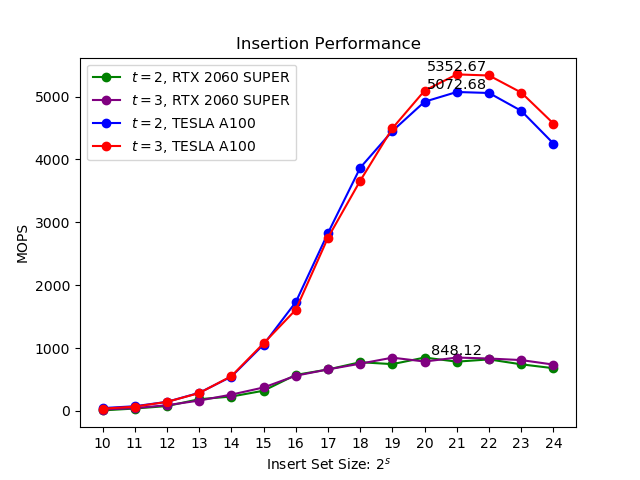
\includegraphics[scale=0.5]{figures/1.png}
    \caption{Experiment 1 Performance}
    \label{fig:experiment1}
\end{figure}

\begin{table}[h]
    \centering
   \begin{tabular}{@{}c|ccccccc@{}}
\toprule
$s$  & $t$ & MOPS    & Time (ms)& StdDev  \\ \midrule
$10$ & 2   & 7.446709  & 0.137510 & 0.063818 \\
$11$ & 2   & 37.200651 & 0.055053 & 0.027095 \\
$12$ & 2   & 76.472696 & 0.053562 & 0.016374 \\
$13$ & 2   &185.561035 & 0.044147 & 0.015856 \\
$14$ & 2   &227.859371& 0.071904 & 0.013538 \\
$15$ & 2   &320.661368& 0.102189 & 0.049058 \\
$16$ & 2   &572.194902& 0.114534 & 0.009390 \\ 
$17$ & 2   &658.499736& 0.199046 & 0.009860 \\ 
$18$ & 2   &773.983850& 0.338694 & 0.005635 \\ 
$19$ & 2   &743.422896& 0.705235 & 0.137846 \\ 
$20$ & 2   &\textbf{848.028746}& 1.236486 & 0.004866 \\ 
$21$ & 2   &782.824122& 2.678957 & 0.274631 \\ 
$22$ & 2   &818.832553& 5.122298 & 0.240417 \\ 
$23$ & 2   &740.279704& 11.331674& 0.807136 \\ 
$24$ & 2   &678.550312& 24.725088& 0.903823\\ 
\bottomrule
\end{tabular}
    \caption{Insertion test on NVIDIA GeForce RTX 2060 SUPER using $t = 2$ hash functions}
    \label{tab:insert_2_2060}
\end{table}

\begin{table}[h]
    \centering
   \begin{tabular}{@{}c|ccccccc@{}}
\toprule
$s$  & $t$ & MOPS    & Time (ms)& StdDev  \\ \midrule
10 & 3 & 21.214532 & 0.048269 & 0.009736 \\
11 & 3 & 44.071065 & 0.046470 & 0.002681 \\
12 & 3 & 90.026727 & 0.045498 & 0.004228 \\
13 & 3 & 164.018451 & 0.049946 & 0.009279 \\
14 & 3 & 258.638111 & 0.063347 & 0.005503 \\
15 & 3 & 371.984887 & 0.088090 & 0.015388 \\
16 & 3 & 559.348878 & 0.117165 & 0.003982 \\
17 & 3 & 659.666305 & 0.198694 & 0.017240 \\
18 & 3 & 750.733137 & 0.349184 & 0.026919 \\
19 & 3 & 846.473374 & 0.619379 & 0.001562 \\
20 & 3 & 784.772035 & 1.336154 & 0.234942 \\
21 & 3 & \textbf{848.118706} & 2.472710 & 0.099679 \\
22 & 3 & 832.881107 & 5.035898 & 0.234401 \\
23 & 3 & 807.912957 & 10.383059 & 0.109445 \\
24 & 3 & 736.136639 & 22.790899 & 0.155948 \\
\bottomrule
\end{tabular}
    \caption{Insertion test on NVIDIA GeForce RTX 2060 SUPER using $3$ hash functions}
    \label{tab:insert_3_2060}
\end{table}

We can find that using $3$ hash functions performs better than using $2$ hash functions in most cases because fewer evictions are needed when using $3$ hash functions. $3$ hash function performs especially better when $s$ is larger, when $s = 24$ the difference is extremely obvious.

\begin{table}[h]
    \centering
   \begin{tabular}{@{}c|ccccccc@{}}
\toprule
$s$  & $t$ & MOPS    & Time (ms)& StdDev  \\ \midrule
10 & 2 & 44.211108 & 0.023162 & 0.003254 \\
11 & 2 & 73.613987 & 0.027821 & 0.002437 \\
12 & 2 & 143.465591 & 0.028550 & 0.002464 \\
13 & 2 & 286.802600 & 0.028563 & 0.002506 \\
14 & 2 & 545.028746 & 0.030061 & 0.000516 \\
15 & 2 & 1055.452489 & 0.031046 & 0.000901 \\
16 & 2 & 1730.606726 & 0.037869 & 0.002185 \\
17 & 2 & 2829.120113 & 0.046330 & 0.001364 \\
18 & 2 & 3867.799868 & 0.067776 & 0.003297 \\
19 & 2 & 4452.415964 & 0.117754 & 0.001905 \\
20 & 2 & 4918.495447 & 0.213190 & 0.001987 \\
21 & 2 & 5072.681438 & 0.413421 & 0.001089 \\
22 & 2 & \textbf{5057.063274} & 0.829395 & 0.002853 \\
23 & 2 & 4773.093010 & 1.757478 & 0.002250 \\
24 & 2 & 4252.760722 & 3.945018 & 0.004734 \\
\bottomrule
\end{tabular}
    \caption{Insertion test on NVIDIA TESLA A100 40GB PCIe using $t = 2$ hash functions}
    \label{tab:insert_2_A100}
\end{table}

\begin{table}[h]
    \centering
   \begin{tabular}{@{}c|ccccccc@{}}
\toprule
$s$  & $t$ & MOPS    & Time (ms)& StdDev  \\ \midrule
10 & 3 & 34.453057 & 0.029722 & 0.001653 \\
11 & 3 & 67.100022 & 0.030522 & 0.001605 \\
12 & 3 & 142.793397 & 0.028685 & 0.003427 \\
13 & 3 & 283.248506 & 0.028922 & 0.000490 \\
14 & 3 & 551.724145 & 0.029696 & 0.001909 \\
15 & 3 & 1073.600350 & 0.030522 & 0.001782 \\
16 & 3 & 1609.303782 & 0.040723 & 0.001657 \\
17 & 3 & 2755.651233 & 0.047565 & 0.002297 \\
18 & 3 & 3661.065435 & 0.071603 & 0.003161 \\
19 & 3 & 4495.664528 & 0.116621 & 0.004782 \\
20 & 3 & 5094.368927 & 0.205830 & 0.003153 \\
21 & 3 & \textbf{5352.674049} & 0.391795 & 0.003084 \\
22 & 3 & 5335.417389 & 0.786125 & 0.001248 \\
23 & 3 & 5063.862307 & 1.656563 & 0.004728 \\
24 & 3 & 4570.751084 & 3.670560 & 0.005147 \\
\bottomrule
\end{tabular}
    \caption{Insertion test on NVIDIA TESLA A100 40GB PCIe using $t = 3$ hash functions}
    \label{tab:insert_3_A100}
\end{table}

With NVIDIA TESLA A100, we get our peak insertion performance of \textbf{5352.674049} millions of insertions per second. The result between different number of hash functions stays the same, that is $t = 3$ performs better than $t = 2$ also due to the decrease in the number of evictions.

We generally get more than $\mathbf{6\times}$ speedup on TESLA A100 with respected to RTX 2060 SUPER, which shows that our implementation obtain an excellent scalability because we mainly benefit from the GPU memory bandwidth and the HBM2e is $3.47$ times as fast as GDDR6 while A100 takes $2.7$ times higher in TFLOPS.


\subsection{Experiment 2: Lookup}

\begin{figure}[h]
    \centering
    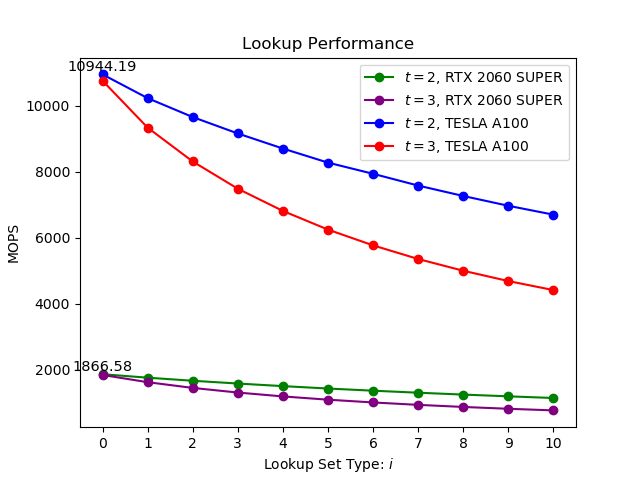
\includegraphics[scale=0.5]{figures/2.png}
    \caption{Experiment 2 Performance}
    \label{fig:experiment2}
\end{figure}

\begin{table}[h]
    \centering
   \begin{tabular}{@{}c|ccccccc@{}}
\toprule
$i$ & $t$ & MOPS    & Time (ms)& StdDev  \\ \midrule
0 & 2 & \textbf{1866.584072} & 8.988192 & 0.107335 \\
1 & 2 & 1761.835282 & 9.522579 & 0.007990 \\
2 & 2 & 1668.597444 & 10.054682 & 0.004976 \\
3 & 2 & 1584.623803 & 10.587507 & 0.003354 \\
4 & 2 & 1506.272597 & 11.138234 & 0.001299 \\
5 & 2 & 1433.399665 & 11.704493 & 0.008614 \\
6 & 2 & 1367.833913 & 12.265536 & 0.005892 \\
7 & 2 & 1306.748787 & 12.838899 & 0.005308 \\
8 & 2 & 1249.908829 & 13.422752 & 0.004688 \\
9 & 2 & 1197.400414 & 14.011366 & 0.002645 \\
10 & 2 & 1146.550585 & 14.632774 & 0.057043 \\
0 & 3 & \textbf{1843.989880} & 9.098323 & 0.002369 \\
1 & 3 & 1625.353454 & 10.322195 & 0.002685 \\
2 & 3 & 1452.115347 & 11.553639 & 0.010561 \\
3 & 3 & 1311.857373 & 12.788902 & 0.005694 \\
4 & 3 & 1194.372580 & 14.046886 & 0.010308 \\
5 & 3 & 1095.647198 & 15.312608 & 0.003277 \\
6 & 3 & 1011.771790 & 16.582016 & 0.004829 \\
7 & 3 & 939.055437 & 17.866055 & 0.005416 \\
8 & 3 & 875.845898 & 19.155443 & 0.005154 \\
9 & 3 & 820.318196 & 20.452083 & 0.006410 \\
10 & 3 & 771.261283 & 21.752960 & 0.007894 \\
\bottomrule
\end{tabular}
    \caption{Lookup test on NVIDIA GeForce RTX 2060 SUPER using $2$ and $3$ hash functions}
    \label{tab:lookup_2060}
\end{table}


\begin{table}[!h]
    \centering
   \begin{tabular}{@{}c|ccccccc@{}}
\toprule
$i$ & $t$ & MOPS    & Time (ms)& StdDev  \\ \midrule
0 & 2 & \textbf{10944.190395} & 1.532979 & 0.001634 \\
1 & 2 & 10225.301127 & 1.640755 & 0.033481 \\
2 & 2 & 9652.516268 & 1.738118 & 0.039536 \\
3 & 2 & 9155.470175 & 1.832480 & 0.039523 \\
4 & 2 & 8699.132169 & 1.928608 & 0.042077 \\
5 & 2 & 8272.762610 & 2.028006 & 0.048818 \\
6 & 2 & 7935.005113 & 2.114330 & 0.025525 \\
7 & 2 & 7577.905498 & 2.213965 & 0.029892 \\
8 & 2 & 7263.175951 & 2.309901 & 0.026111 \\
9 & 2 & 6966.356637 & 2.408320 & 0.027162 \\
10 & 2 & 6697.239074 & 2.505094 & 0.027777 \\
0 & 3 & \textbf{10752.596504} & 1.560294 & 0.019172 \\
1 & 3 & 9331.956724 & 1.797824 & 0.045214 \\
2 & 3 & 8307.342176 & 2.019565 & 0.055082 \\
3 & 3 & 7482.538448 & 2.242182 & 0.065040 \\
4 & 3 & 6810.226405 & 2.463533 & 0.072663 \\
5 & 3 & 6244.869361 & 2.686560 & 0.083055 \\
6 & 3 & 5768.100057 & 2.908621 & 0.093335 \\
7 & 3 & 5354.653074 & 3.133203 & 0.101179 \\
8 & 3 & 4998.941599 & 3.356154 & 0.112646 \\
9 & 3 & 4687.387080 & 3.579226 & 0.121195 \\
10 & 3 & 4413.198677 & 3.801600 & 0.130535 \\
\bottomrule
\end{tabular}
    \caption{Lookup test on NVIDIA TESLA A100 using $2$ and $3$ hash functions}
    \label{tab:lookup_A100}
\end{table}

From table \ref{tab:lookup_2060} and \ref{tab:lookup_A100} we can find that for the lookup test, time increases as $i$ increases because more elements are not in the hash table as $i$ becomes bigger. The lookup time in Cuckoo Hashing is $O(t)$ when the element we try to lookup is already in the hash table, then it will take less than $t$ steps to find that key. Otherwise, it will take the whole $t$ step to give a not found.

Therefore, the performance of lookup reaches the peak when all the lookup keys are in the hash table. While all the keys are not in the hash table, it takes the longest time but the time complexity is still a constant because the number of hash functions $t$ is a constant. And when $t$ is smaller, the performance is better. However, smaller $t$ may increase the number of evictions in insertion. So, in practice we need balance between insertion and lookup.

According to Table \ref{tab:lookup_A100}, we get a peak performance of $\mathbf{10944.190395}$ millions of lookups per second with NVIDIA TESLA A100, which is extremely fast while in the worst case all the lookups are done in $2.51\text{ms}$ when $t = 2$. In addition, our implementation still obtains an excellent in the lookup, reaching a speedup of more $\mathbf{6 \times}$ with respected to RTX 2060 SUPER.

\subsection{Experiment 3: Size}

\begin{figure}[!h]
    \centering
    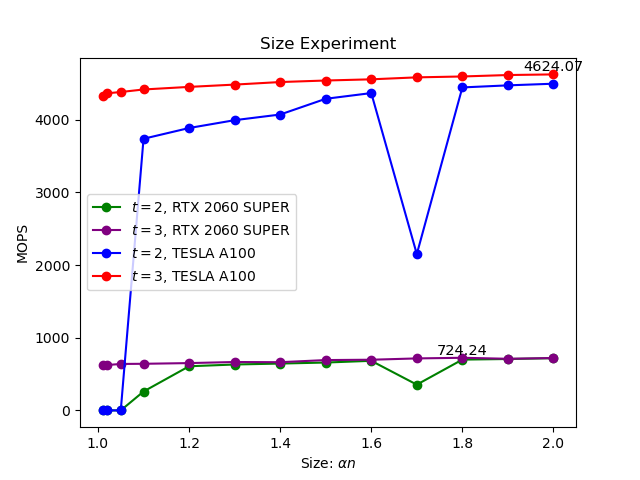
\includegraphics[scale=0.5]{figures/3.png}
    \caption{Experiment 3: Size Test}
    \label{fig:experiment3}
\end{figure}

\begin{table}[h]
    \centering
   \begin{tabular}{@{}c|ccccccc@{}}
\toprule
$s$ & $t$ & MOPS    & Time (ms)& StdDev  \\ \midrule
2.0 & 2 & \textbf{718.569511} & 23.348077 & 0.526595 \\
1.9 & 2 & 707.180415 & 23.724096 & 0.583006 \\
1.8 & 2 & 699.033878 & 24.000576 & 0.654333 \\
1.7 & 2 & 354.465352 & 47.331046 & 1.299906 \\
1.6 & 2 & 682.258901 & 24.590688 & 0.316653 \\
1.5 & 2 & 658.699933 & 25.470195 & 0.726411 \\
1.4 & 2 & 644.583205 & 26.028007 & 0.887359 \\
1.3 & 2 & 631.628612 & 26.561837 & 0.594943 \\
1.2 & 2 & 607.410984 & 27.620864 & 0.922161 \\
1.1 & 2 & 259.893430 & 64.554214 & 1.874496 \\
1.05 & 2 & N/A & N/A & N/A \\
1.02 & 2 & N/A & N/A & N/A \\
1.01 & 2 & N/A & N/A & N/A \\
\bottomrule
\end{tabular}
    \caption{Size test on NVIDIA GeForce RTX 2060 SUPER using $2$ hash functions}
    \label{tab:size_2_2060}
\end{table}

\begin{table}[h]
    \centering
   \begin{tabular}{@{}c|ccccccc@{}}
\toprule
$s$ & $t$ & MOPS    & Time (ms)& StdDev  \\ \midrule
2.0 & 3 & \textbf{720.760163} & 23.277113 & 0.823124 \\
1.9 & 3 & 710.266831 & 23.621004 & 0.795786 \\
1.8 & 3 & 724.240721 & 23.165248 & 0.162821 \\
1.7 & 3 & 715.366934 & 23.452602 & 0.253312 \\
1.6 & 3 & 697.417215 & 24.056211 & 0.665444 \\
1.5 & 3 & 692.596413 & 24.223654 & 0.630849 \\
1.4 & 3 & 663.355432 & 25.291443 & 0.560652 \\
1.3 & 3 & 665.923213 & 25.193920 & 0.797485 \\
1.2 & 3 & 651.055876 & 25.769241 & 0.822991 \\
1.1 & 3 & 641.431637 & 26.155891 & 0.766913 \\
1.05 & 3 & 639.108578& 26.250964 & 0.603821 \\
1.02 & 3 & 624.410461& 26.868890 & 0.688250 \\
1.01 & 3 & 622.909822& 26.933619 & 0.796268 \\
\bottomrule
\end{tabular}
    \caption{Size test on NVIDIA GeForce RTX 2060 SUPER using $3$ hash functions}
    \label{tab:size_3_2060}
\end{table}

\begin{table}[h]
    \centering
   \begin{tabular}{@{}c|ccccccc@{}}
\toprule
$s$ & $t$ & MOPS    & Time (ms)& StdDev  \\ \midrule
2.0 & 2 & \textbf{4495.988473} & 3.731597 & 0.047658 \\
1.9 & 2 & 4473.218103 & 3.750592 & 0.043783 \\
1.8 & 2 & 4444.836303 & 3.774541 & 0.045024 \\
1.7 & 2 & 2150.872191 & 7.800192 & 0.070234 \\
1.6 & 2 & 4367.152402 & 3.841683 & 0.043648 \\
1.5 & 2 & 4288.401832 & 3.912230 & 0.090330 \\
1.4 & 2 & 4071.855181 & 4.120288 & 0.041169 \\
1.3 & 2 & 3994.070087 & 4.200531 & 0.038393 \\
1.2 & 2 & 3886.171126 & 4.317158 & 0.040137 \\
1.1 & 2 & 3738.228285 & 4.488013 & 0.003802 \\
1.05 & 2 & N/A & N/A & N/A \\
1.02 & 2 & N/A & N/A & N/A \\
1.01 & 2 & N/A & N/A & N/A \\
\bottomrule
\end{tabular}
    \caption{Size test on NVIDIA TESLA A100 using $2$ hash functions}
    \label{tab:size_2_A100}
\end{table}

\begin{table}[!h]
    \centering
   \begin{tabular}{@{}c|ccccccc@{}}
\toprule
$s$ & $t$ & MOPS    & Time (ms)& StdDev  \\ \midrule
2.0 & 3 & \textbf{4624.068615} & 3.628237 & 0.044546 \\
1.9 & 3 & 4615.325053 & 3.635110 & 0.045759 \\
1.8 & 3 & 4595.526630 & 3.650771 & 0.045174 \\
1.7 & 3 & 4583.313615 & 3.660499 & 0.048979 \\
1.6 & 3 & 4556.363571 & 3.682150 & 0.045424 \\
1.5 & 3 & 4539.911130 & 3.695494 & 0.052675 \\
1.4 & 3 & 4518.867180 & 3.712704 & 0.049443 \\
1.3 & 3 & 4483.699920 & 3.741824 & 0.043908 \\
1.2 & 3 & 4452.022667 & 3.768448 & 0.038733 \\
1.1 & 3 & 4416.581690 & 3.798688 & 0.038431 \\
1.05 & 3 & 4381.700577 & 3.828928 & 0.044611 \\
1.02 & 3 & 4364.069773 & 3.844397 & 0.044340 \\
1.01 & 3 & 4328.415614 & 3.876064 & 0.053024 \\
\bottomrule
\end{tabular}
    \caption{Size test on NVIDIA TESLA A100 using $3$ hash functions}
    \label{tab:size_3_A100}
\end{table}

According to Figure \ref{fig:experiment3}, we can see that generally, the performance increases as the size increases because there will be less evictions and rehashes. 

When size is $1.7n$, we get a performance drop because we encounter one rehash in this test key set. When the size $\leq 1.05n$ and if we choose $2$ hash functions, the hash table will infinitely rehash.\\

When we choose $3$ hash functions, there will not be any rehash and the performance increases as the size increases due to fewer evictions.

According to Figure \ref{fig:experiment3} and Table \ref{tab:size_3_A100}, on NVIDIA TESLA A100, we get our peak performance of \textbf{4624.068615} with $3$ hash functions and size of $2.0n$.

\subsection{Experiment 4: Bound}

I test Cuckoo Hashing with different bounds of $l \log n$ on the maximum length of eviction chain before restarting.

\begin{figure}[h]
    \centering
    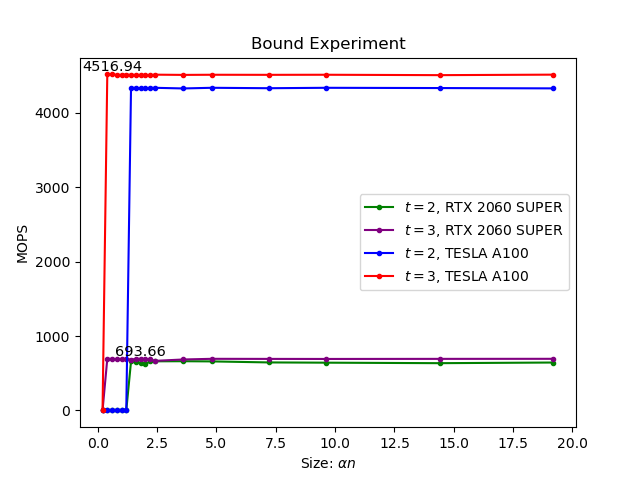
\includegraphics[scale=0.5]{figures/4.png}
    \caption{Experiment 4: Bound Test}
    \label{fig:experiment4}
\end{figure}

\vspace{1.23pt}

\begin{table}[!h]
    \centering
   \begin{tabular}{@{}c|ccccccc@{}}
\toprule
$l$ & $t$ & MOPS    & Time (ms)& StdDev  \\ \midrule
0.2 & 2 & N/A & N/A & N/A \\
0.4 & 2 & N/A & N/A & N/A \\
0.6 & 2 & N/A & N/A & N/A \\
0.8 & 2 & N/A & N/A & N/A \\
1.0 & 2 & N/A & N/A & N/A \\
1.2 & 2 & N/A & N/A & N/A \\
1.4 & 2 & 4336.226983 & 3.869082 & 0.040889 \\
1.6 & 2 & \textbf{4336.965930} & 3.868422 & 0.041448 \\
1.8 & 2 & 4329.588092 & 3.875014 & 0.037551 \\
2.0 & 2 & 4331.934797 & 3.872915 & 0.037947 \\
2.2 & 2 & 4335.932864 & 3.869344 & 0.038864 \\
2.4 & 2 & 4336.851103 & 3.868525 & 0.040728 \\
3.6 & 2 & 4328.079694 & 3.876365 & 0.038323 \\
4.8 & 2 & 4336.937169 & 3.868448 & 0.042185 \\
7.2 & 2 & 4331.211905 & 3.873562 & 0.038510 \\
9.6 & 2 & 4336.786582 & 3.868582 & 0.043544 \\
14.4 & 2 & 4333.388402 & 3.871616 & 0.038374 \\
19.2 & 2 & 4329.037487 & 3.875507 & 0.046952 \\
\bottomrule
\end{tabular}
    \caption{Bound test on NVIDIA TESLA A100 using $2$ hash functions}
    \label{tab:bound_2_A100}
\end{table}

\newpage

From the Table \ref{tab:bound_2_A100}, \ref{tab:bound_3_A100}, \ref{tab:bound_2_2060}, \ref{tab:bound_3_2060} and Figure \ref{fig:experiment4}, we can see that when choosing $2$ hash functions, the performance remains almost the same after $l \geq 1.4$ (bound length $\geq 1.4 \log n$).

When choosing $3$ hash functions, we only need $l \geq 0.4$ to get a good performance. 

The best bound in our experiment is bolded in the table.

\begin{table}[!h]
    \centering
   \begin{tabular}{@{}c|ccccccc@{}}
\toprule
$l$ & $t$ & MOPS    & Time (ms)& StdDev  \\ \midrule
0.2 & 3 & N/A & N/A & N/A \\
0.4 & 3 & \textbf{4516.142393} & 3.714944 & 0.047456 \\
0.6 & 3 & 4516.943821 & 3.714285 & 0.042790 \\
0.8 & 3 & 4511.129706 & 3.719072 & 0.048300 \\
1.0 & 3 & 4511.479023 & 3.718784 & 0.050594 \\
1.2 & 3 & 4514.874533 & 3.715987 & 0.046709 \\
1.4 & 3 & 4511.129590 & 3.719072 & 0.050060 \\
1.6 & 3 & 4511.533343 & 3.718739 & 0.048303 \\
1.8 & 3 & 4511.595532 & 3.718688 & 0.049938 \\
2.0 & 3 & 4509.577610 & 3.720352 & 0.051675 \\
2.2 & 3 & 4509.236274 & 3.720634 & 0.050588 \\
2.4 & 3 & 4513.382040 & 3.717216 & 0.050051 \\
3.6 & 3 & 4510.206033 & 3.719834 & 0.051105 \\
4.8 & 3 & 4512.162369 & 3.718221 & 0.051948 \\
7.2 & 3 & 4511.051972 & 3.719136 & 0.047064 \\
9.6 & 3 & 4512.240083 & 3.718157 & 0.048978 \\
14.4 & 3 & 4506.902747 & 3.722560 & 0.047575 \\
19.2 & 3 & 4513.622961 & 3.717018 & 0.050403 \\
\bottomrule
\end{tabular}
    \caption{Bound test on NVIDIA TESLA A100 using $3$ hash functions}
    \label{tab:bound_3_A100}
\end{table}

\begin{table}[!h]
    \centering
   \begin{tabular}{@{}c|ccccccc@{}}
\toprule
$l$ & $t$ & MOPS    & Time (ms)& StdDev  \\ \midrule
0.2 & 2 & N/A & N/A & N/A \\
0.4 & 2 & N/A & N/A & N/A \\
0.6 & 2 & N/A & N/A & N/A \\
0.8 & 2 & N/A & N/A & N/A \\
1.0 & 2 & N/A & N/A & N/A \\
1.2 & 2 & N/A & N/A & N/A \\
1.4 & 2 & 657.483519 & 25.517318 & 0.312952 \\
1.6 & 2 & 646.936886 & 25.933312 & 0.659120 \\
1.8 & 2 & 641.007204 & 26.173210 & 0.573636 \\
2.0 & 2 & 620.847396 & 27.023092 & 0.606418 \\
2.2 & 2 & 658.149056 & 25.491514 & 0.317434 \\
2.4 & 2 & 659.814903 & 25.427155 & 0.147894 \\
3.6 & 2 & \textbf{661.132839} & 25.376468 & 0.109419 \\
4.8 & 2 & 658.687197 & 25.470688 & 0.214283 \\
7.2 & 2 & 644.927489 & 26.014112 & 0.493037 \\
9.6 & 2 & 641.568838 & 26.150298 & 0.707538 \\
14.4 & 2 & 634.861433 & 26.426579 & 0.982739 \\
19.2 & 2 & 643.584807 & 26.068384 & 0.742324 \\
\bottomrule
\end{tabular}
    \caption{Bound test on NVIDIA 2060 SUPER using $2$ hash functions}
    \label{tab:bound_2_2060}
\end{table}

\begin{table}[!h]
    \centering
   \begin{tabular}{@{}c|ccccccc@{}}
\toprule
$l$ & $t$ & MOPS    & Time (ms)& StdDev  \\ \midrule
0.2 & 3 & N/A & N/A & N/A \\
0.4 & 3 & 693.425597 & 24.194688 & 0.115743 \\
0.6 & 3 & 693.467047 & 24.193242 & 0.116118 \\
0.8 & 3 & 690.305337 & 24.304051 & 0.234168 \\
1.0 & 3 & 693.034023 & 24.208358 & 0.143322 \\
1.2 & 3 & 693.265324 & 24.200282 & 0.120261 \\
1.4 & 3 & 681.274671 & 24.626214 & 0.550600 \\
1.6 & 3 & 693.066273 & 24.207232 & 0.109783 \\
1.8 & 3 & \textbf{693.658439} & 24.186567 & 0.115933 \\
2.0 & 3 & 691.121569 & 24.275347 & 0.161366 \\
2.2 & 3 & 685.183113 & 24.485741 & 0.552498 \\
2.4 & 3 & 665.937249 & 25.193389 & 0.589150 \\
3.6 & 3 & 684.540419 & 24.508730 & 0.585207 \\
4.8 & 3 & 693.442664 & 24.194093 & 0.113214 \\
7.2 & 3 & 692.317996 & 24.233396 & 0.213677 \\
9.6 & 3 & 691.614976 & 24.258029 & 0.131916 \\
14.4 & 3 & 692.744288 & 24.218483 & 0.133526 \\
19.2 & 3 & 693.520618 & 24.191373 & 0.115917 \\
\bottomrule
\end{tabular}
    \caption{Bound test on NVIDIA 2060 SUPER using $3$ hash functions}
    \label{tab:bound_3_2060}
\end{table}


% \begin{strip}
% \centering
% \begin{tabular}{@{}c|ccccccc@{}}
% \toprule
% Graph            & Single Thread  & Topdown, threads     & Hybrid, threads      & \textbf{Speedup} & Time (s) & StdDev \\ \midrule
% web-Stanford     & 227.185 & 675.243, 4  & 648.741, 5  & 2.972 & 0.00342469 & 1.38624    \\
% roadNet-CA       & 63.536  & 208.959, 4  & 204.252, 4  & 3.289  & 0.0274864 & 0.552123 \\
% com-Orkut        & 373.057 & \textbf{5291.94, 64} & 5280.75, 64 & 14.185 & 0.0225889 & 99.7608 \\
% soc-Livejournal1 & 72.3957 & 1439.49, 63 & 1439.56, 63 & 19.885 & 0.047927 & 15.9759 \\
% RMAT1            & 18.965 & 559.64, 63  & 549.926, 64 & \textbf{29.526} & 1.78583 & 6.17689  \\
% RMAT2            & 33.6309 &    906.489, 64         &   912.044, 64          &   27.119 & 1.09644 & 11.5889      \\
% RMAT3            &    138.81     & 2293.06, 62            & 2307.07, 63            &16.620 & 0.43345 & 1000.97         \\ \bottomrule
% \end{tabular}

% \end{strip}

% The performance are measured in MTEPS (millions of edges traversed per second), the baseline is the conventional top-down with single thread. We can find that the hybrid method only performs a little better in some graphs, it cannot significantly increase the peak performance. However, in the experiments, I find that the hybrid method can perform better in many thread nums.\\
% In the first two graphs, our peak speedup is around $3$, I think this is because the average degree of the graph is not much enough and the graph is also much smaller than the rest, we reach the peak performance using just $4$ threads.\\
% In the third graph, com-Orkut, our algorithm reach the peak performance of $5291.94$ MTEPS, which is very efficient. And in the experiment, our performance is always increasing as the number of threads increase.\\
% In the soc-Livejournal1 graph, we also obtain a relatively good speedup.\\
% For the three big random graph, the absolute performance in MTEPS is not that high because of memory access, these graph need too much memory and the cache performance is not that good. However, our algorithm gains a very good speedup in these graphs. The performance almost always increases as the number of threads increase.\\
% And in these graphs, we reach our peak speedup of $29.526$, which is good enough and our algorithm is efficient.

% \begin{strip}
%     \centering
%     \includegraphics[scale=0.8]{figures/speedup.png}
% \end{strip}

\newpage

\bibliography{bibliography}

% All the experiment data are listed on the next page.

% \begin{figure}[h]
%     \centering
%     \includegraphics[scale=0.5]{figures/web-Stanford.png}
%     \caption{web-Stanford Performance}
%     \label{fig:web-Stanford}
%     The graph is too small that we reach peak performance within only $4$ threads with speedup of $2.972$.
% \end{figure}

% \begin{figure}[h]
%     \centering
%     \includegraphics[scale=0.5]{figures/roadNet-CA.png}
%     \caption{roadNet-CA Performance}
%     \label{fig:roadNet-CA}
%     The graph is too small that we reach peak performance within only $4$ threads with speedup of $3.289$.
% \end{figure}

% \begin{figure}[h]
%     \centering
%     \includegraphics[scale=0.5]{figures/soc-LiveJournal1.png}
%     \caption{soc-LiveJournal1 Performance}
%     \label{fig:soc-LiveJournal1}
% \end{figure}


% \begin{figure}[h]
%     \centering
%     \includegraphics[scale=0.5]{figures/com-Orkut.png}
%     \caption{com-Orkut Performance}
%     \label{fig:com-Orkut}
% \end{figure}

% \begin{figure}[h]
%     \centering
%     \includegraphics[scale=0.5]{figures/RMAT1.png}
%     \caption{RMAT1 Performance}
%     \label{fig:RMAT1}
% \end{figure}


% \begin{figure}[h]
%     \centering
%     \includegraphics[scale=0.5]{figures/RMAT2.png}
%     \caption{RMAT2 Performance}
%     \label{fig:RMAT2}
% \end{figure}

% \begin{figure}[h]
%     \centering
%     \includegraphics[scale=0.5]{figures/RMAT3.png}
%     \caption{RMAT3 Performance}
%     \label{fig:RMAT3}
% \end{figure}



\end{document}
